
\chapter{Software Architektur}
\section{Anforderungen}
\label{sec:Anforderungen} 
%Christoph

Im Folgenden sollen die Anforderungen an die Studienarbeit festgelegt werden. \newline
Ein Hauptbestandteil der Arbeit besteht darin, ein Vorgängerprojekt mit einer AR.Drone 2.0 in das ROS Framework zu portieren.
Dies beinhaltet eine Modularisierung der Projektbestandteile in ROS Nodes. Ziel soll sein, den Quadrocopter mit Hilfe einer Kinect und Gestenerkennung steuern zu können. Anzumerken ist, dass ROS nur unter UNIX basierten Betriebssystemen läuft und das bestehende Projekt Libraries verwendet, welche nur unter Windows verfügbar sind. \newline
Eine weitere Vorgabe besteht darin, dass man neben der realen Drohne jegliche Funktionalität auch in einer Simulation laufen soll. \newline
Somit kann man für Präsentationen, in denen der Flug einer Drohne nicht möglich ist, den Quadrocopter in einer frei gestaltbaren simulierten Umgebung fliegen lassen. \newline
Ein weiterer Bestandteil dieser Arbeit besteht darin, Ansätze und Limitationen der Implementierung eines Assistenzsystems zu testen und zu bewerten. Dafür soll ein externes Projekt, zur Gewinnung von Tiefenbildern aus einer monokularen Kamera, in die Projektumgebung integriert werden. Hierbei soll es wiederum möglich sein, dass die Videostream sowohl von der realen, als auch von der simulierten Drohne gesendet werden kann. \newline
Es soll dabei ermittelt werden, ob die Nutzung der Software für den Anwendungszweck praktikabel und sinnvoll ist.

%hier weitermachen, wenn man weiß wie weit wir tatsächlich kommen #wahrscheinlichsindwirzublöd #forschung>implementierung

%	-> Wände / Türen erkennen
%	-> aktives eingreifen der Drohne in das Geschehen -> Kollisionsvermeidung


\section{Überblick}
\label{Überblick}

\section{Bildverarbeitung}
\label{Bildverarbeitung}
In diesem Abschnitt wird beschrieben, wie Drohne aus den Bildern der Kamera Informationen gewinnen kann, die später für die Betrachtung des Assistenzsystems relevant sind. 
%-> errechnung von bewegungen + tiefenbildanalyse
%basierend auf paper Christian Forster, Matia Pizzoli, Davide Scaramuzza
%In diesem Abschnitt soll die technische Ausführung beschrieben werden.

\subsection{Semi-Direct Monocular Visual Odometry - SVO}


Eine Grundanforderung an das Projekt ist die Nutzung einer nicht modifizierten AR.Drone. Dadurch entsteht die Problematik, dass keine Tiefenbildkamera genutzt werden kann, um in Echtzeit Tiefenbilder zu erhalten. Die Drohne ist lediglich mit einer monokularen \footnote{Monokular ist die Bezeichnung für Kameras mit einer einzelnen Linse} Frontkamera ausgestattet. \newline
Um Tiefeninformationen aus den Bildern einer solchen Kamera zu gewinnen, wird eine Szene aus verschiedenen Perspektiven aufgenommen. Anschließend gibt es unterschiedliche Ansätze um aus den aufeinanderfolgenden Bildern Kamerapositionen und Umgebungsstrukturen zu ermitteln. \newline
Feature basierte Ansätze sind der aktuelle Standard zur Berechnung der Kamerapostion. Diese versuchen die wichtigsten Merkmale eines Bildes, die Features, zu extrahieren. Mit Hilfe von Feature Deskriptor Algorithmen werden Vektoren mit Informationen zu invarianten Bildbereichen berechnet. Diese Vektoren verhalten sich wie ein einzigartiger Fingerabdruck, der die Merkmale repräsentiert. \newline
Aufeinanderfolgende Bilder werden dann mit Hilfe dieser Deskriptoren abgeglichen und sowohl Kamerabewegungen, als auch Strukturen werden rekonstruiert. Zur Optimierung sind abschließend die ermittelten Kamerapositionen anzugleichen. Dies geschieht mit Hilfe von Algorithmen zur Minimierung des Reprojektionsfehlers. \footnote{Reprojektionsfehler sind geometrische Fehler die im Zusammenhang zwischen abgebildeten und berechneten Bildpunkten entstehen.} 
\newline
%\cite{} https://en.wikipedia.org/wiki/Reprojection_error
%Bilder dazu hier einfügen
Ein weiterer Ansatz ist die direkte Methode. Hierbei werden die Features nicht über Deskriptor Algorithmen bestimmt, sondern das Problem wird über die Intensitäten der Pixel gelöst. Bei einem Graustufenbild entspricht diese Intensität der Helligkeit von Bildbereichen. \newline
Somit kann bei der Rekonstruktion im Gegensatz zum Feature basierten Ansatz auch die Richtung der Gradienten von Intensitäten genutzt werden. Dadurch funktioniert diese Methode auch bei Bildern mit sehr wenig Textur, Bewegungsunschärfe und fehlerhaftem Kamerafokus. \newline
Das für diese Arbeit relevante Vorgehen kombiniert die Vorteile der beschriebenen Methoden. Die semi-direkte Odometrie %footnote dazu
verwendet einen Algorithmus der ebenfalls auf Zusammenhängen von Features basiert. Diese werden jedoch implizit aus einer direkten Bewegungsabschätzung bezogen, anstatt explizit durch Algorithmen mit Feature Deskriptoren berechnet zu werden. \newline
Dadurch müssen Features nur extrahiert werden, wenn diese noch nicht auf einem der vorherigen Bildern vorhanden waren. Insgesamt ist dieser Ansatz somit schnell, da wenig Berechnungen pro Bild stattfinden und auf Grund der Verwendung von Intensitätsgradienten äußerst genau und robust. \newline
Diese Eigenschaften sind für die Anforderungen der Studienarbeit essentiell, da die Drohne sich sehr schnell bewegen kann und somit in möglichst kurzer Zeit neue Bilder auswerten muss. Das beschrieben Verfahren minimiert damit die Auswirkungen der typischen Probleme von Drohnen. Diese sind einerseits die niedrige Texturierung der Umgebung, welche hauptsächlich in Innenräumen auftritt und andererseits kameraspezifische Probleme wie Bewegungsunschärfe und der Verlust des Kamerafokus.


\subsection{Kamerakalibrierung}
Ein Grundproblem der Bildverarbeitung ist die Verzerrung des Bildes. 
Da die Bestimmung der Kameraposition möglichst genau sein soll, muss die Kamera vorher kalibriert werden. Dies bedeutet, dass Ungenauigkeiten der Linse erkannt und softwareseitig ausgeglichen werden. Dafür werden die intrinsischen Parameter der Kamera bestimmt \newline

\subsubsection*{Kalibrierungsmodelle}
Hierbei unterstützt SVO drei Kamera Modelle: ATAN, Ocam und Lochkamera. \cite{svo_cameracalibration} \newline
Das ATAN Modell basiert auf dem \textit{Field of View \emph{(FOV)}} Verzerrungsmodell "Straight lines have to be straight [...]" von Devernay und Faugeras.\newline %cite https://hal.inria.fr/inria-00267247/document
Der Vorteil dieser Kalibrierungsmethode ist die äußerst schnelle Berechnung der Projektion des Bildes. % cite https://github.com/uzh-rpg/rpg_svo/wiki/Camera-Calibration
Das Modell vernachlässigt jedoch tangentiale Verzeichnung, welche auftritt, wenn optische und mechanische Bestandteile des Objektives, sowie der CCD-Sensor 
\footnote{CCD steht für \emph{charge-coupled device}, was übersetzt ladungsgekoppeltes Bauteil bedeutet. Dieses lichtempfindliche elektronische Bauteil wird zur Bildaufnahme verwendet.} 
nicht perfekt zueinander ausgerichtet sind. % cite http://www.aishack.in/tutorials/major-physical-defects-cameras/
Weiterhin sollte die Kamera mit einem globalem Shutter ausgestattet sein, um die Extraktion von Bildmerkmalen bei Bewegungen zu gewährleisten. Kameras mit Global-Shutter-CMOS  
\footnote{CMOS steht für \emph{Complementary metal-oxide-semiconductor} und ist ein spezieller Halbleiter der zur Bildaufnahme verwendet wird.} % cite https://de.wikipedia.org/wiki/Complementary_metal-oxide-semiconductor
Sensoren und CCD-Sensoren nehmen Bild nicht zeilen- und spaltenweise, sondern vollständig auf und sind daher für das Verfahren geeignet. \newline
Die Drohne besitzt eine veraltete und günstige Kamera mit einem CMOS Sensor, wodurch sowohl tangentiale Verzerrung, als auch der Rolling-Shutter-Effekt auftreten können. \newline
%cite https://dspace.cvut.cz/bitstream/handle/10467/66885/F3-DP-2017-Pahorecky-Petr-priloha-ARDrone_Developer_Guide.pdf?sequence=-1&isAllowed=y
Daher ist das ATAN Modell zwar eine der besten Kalibrierungsmethoden für teure Hochleistungskameras, jedoch ist es für die Betrachtungen dieser Arbeit nicht optimal. \newline
Der zweite Ansatz zur Kalibrierung ist das Ocam Modell von Davide Scaramuzza. Diese Methode sollte für Kameras mit sehr weitem Sichtfeld, oder omnidirektionalen Kameras genutzt werden. Damit ist es für die Drohne nicht geeignet. \newline
Die dritte unterstützte Kalibrierungsmethode ist das Modell der Lochkamera.
Hierbei handelt es sich um den aktuellen Standard in OpenCV \footnote{``OpenCV is the leading open source library for computer vision, image processing and machine learning, and now features GPU acceleration for real-time operation.''} %cite https://developer.nvidia.com/opencv
und ROS. Hierbei wird die Verzerrung mit Hilfe von fünf intrinsischen Parametern beschrieben, welche im Rahmen der Kalibrierung bestimmt werden müssen.

\begin{figure}[ht]
	\centering
	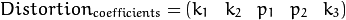
\includegraphics[scale=0.7]{Bilder/distortion.png}
	\label{fig:distortion}
\end{figure}

OpenCV betrachtet dabei radiale und tangentiale Faktoren. Die Formel für radiale Verzeichnung ist die Folgende:

\begin{figure}[ht]
	\centering
	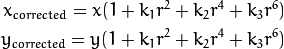
\includegraphics[scale=0.7]{Bilder/radialFactors.png}
	\label{fig:radial}
\end{figure}

Hierbei wird aus einem alten Bildpunkt $(x,y)$ des Eingabebildes die korrigierte Position $x_{corrected} y_{corrected}$ bestimmt. \newline
Die Berechnung der tangentialen Verzerrung erfolgt durch die Formel:

\begin{figure}[ht]
	\centering
	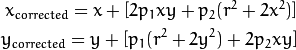
\includegraphics[scale=0.7]{Bilder/tangentialFactors.png}
	\label{fig:radial}
\end{figure}

Abschließend werden die Einheiten angepasst:

\begin{figure}[ht]
	\centering
	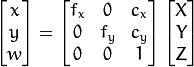
\includegraphics[scale=0.7]{Bilder/matrixEquation.png}
	\label{fig:radial}
\end{figure}

Dabei entspricht $f_x$ und $f_y$ der Brennweite der Linse und $c_x$, sowie $c_y$ beschreiben die optische Bildmitte in Pixelkoordinaten. \newline
% cite http://docs.opencv.org/2.4/doc/tutorials/calib3d/camera_calibration/camera_calibration.html
Dieser Ansatz ist der einfachste und funktioniert grundsätzlich mit jeder Kamera.

\subsubsection*{Umsetzung der Kalibrierung}
Um die intrinsischen Parameter der Kamera zu bestimmen, wird ein bekanntes Bild oder Muster aufgenommen. Dazu wird ein Vergleich zwischen den theoretischen und tatsächlichen Abmessungen angestellt. Hierzu wird meist ein einfaches Schachbrettmuster genutzt, welches im möglichst vielen verschiedenen Perspektiven aufgenommen wird. Bei der realen Drohne wird dazu das Muster ausgedruckt, bei der Simulation muss hingegen ein muss ein solches Objekt in die Welt eingefügt werden. Da die Kamera in der Simulation ohnehin keine intrinsischen Fehler aufweisen sollte, kann auf eine Kalibrierung verzichtet werden. \newline

\begin{figure}[ht]
	\centering
	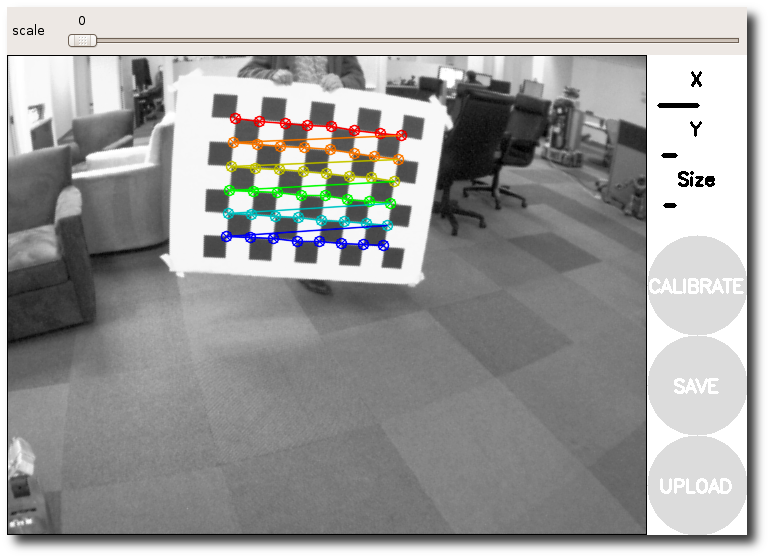
\includegraphics[scale=0.4]{Bilder/calibrationChecker.png}
	\label{fig:calibrationChecker}
\end{figure}

Die Kalibrierung wurde mit dem frei verfügbaren ROS Node \textit{camera\_calibration} umgesetzt. Das Ergebnis ist abhängig von der Anzahl der Perspektiven und der Qualität der Aufnahmen. Aufgegeben wird dann die List der Parameter, die für das Lochkamera Modell notwendig sind.

\subsection{Regularized Monocular Depth Estimation - REMODE}

%todo Remode ausformulieren

Im vorherigen Abschnitt wurde beschrieben, wie anhand von aufeinanderfolgenden Bildern die Position der Kamera im Raum bestimmt werden kann. Dieses Problem wird seit mehr als 20 Jahren untersucht und wird als Structure From Motion \emph{SFM} in der Bildverarbeitung und Simultaneous Localization and Mapping \emph{SLAM} in der Robotik bezeichnet. \newline
%Smith, R.C.; Cheeseman, P. (1986). "On the Representation and Estimation of Spatial Uncertainty" (PDF). The International Journal of Robotics Research. 5 (4): 56–68. 
Um den Nutzer aktiv bei der Steuerung der Drohne zu unterstützen werden jedoch Tiefeninformationen benötigt. Dazu müssen Tiefenbilder und Tiefenkarten (footnote) aus den Bildern der monokularen Kamera bestimmt werden. \newline
Für diesen Schritt gibt es unterschiedliche Ansätze. Der State of the Art ist die Tiefenschätzung mit Hilfe der 


berechnung in echtzeit auf pixelbasis

live feedback wie hoch die Fehlerrate und Genauigkeit der bestimmten Tiefeninformationen ist

Nutzung des opensource projects REMODE - Implementation basierend auf dem Paper von Matia Pizzoli, Christian Forster und Davide Scaramuzza

kombiniert Bayes Tiefenschätzungen basierend auf der Artbeit von [19] und neueste Entwicklungen in Konvexoptimierung


\begin{figure}[ht]
	\centering
	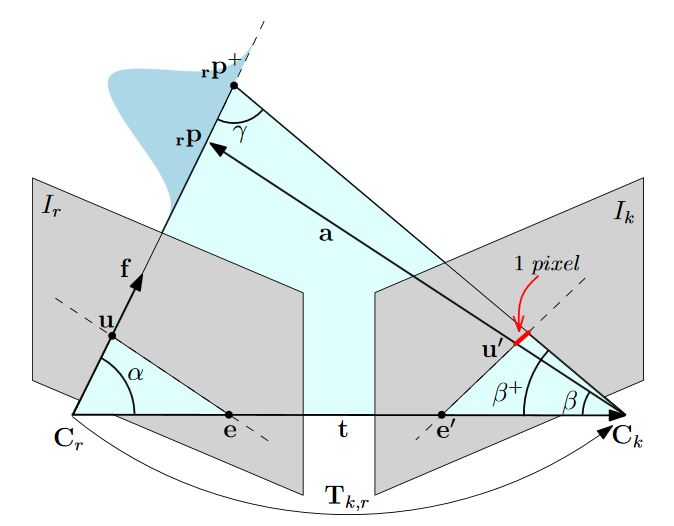
\includegraphics[scale=0.7]{Bilder/REMODE_overview.jpg}
	\label{fig:radial}
\end{figure}

starre Transformation eines Körpers Tk,r 
Kamerapositionen Ir und Ik mit den Kamerazentren Cr und Ck
Aktuelle Schätzung eines Punktes der Szene rP auf der epipolaren fläche
Varianz von einem Pixel auf der epipolaren Linie durch e strich und u strich als T2 = () siehe arbeit

genaue implementationsdetails können im Paper (quelle) nachgeschaut werden - übersteigen aufgrund der hohen mathematischen und bildverarbeitungstechnischen Komplexität den Umfang dieser Arbeit

zusammenspiel von SVO und REMODE für handelsüblichen Laptop mit CPU und GPU geeignet
SVO läuft komplett auf CPU, REMODE mit GPU auf Nvidia CUDA (footnote)
Implemtation von REMODE setzt auf eine durchschnittliche Bewegung der Kamera um 0.0038 meter pro sekunde, durchschnittliche
Tiefe von 1 meter und berechnungszeit von 3.3 ms pro Bild

\subsection{Kinect}
%Max
\subsection{Die einzelnen ROS Nodes}
%Beide
\subsection{Architektur}
%Beide



%Bild der Drohne http://lightspots.ch/images/ARdronebw.png
%Bild vom Typ https://img.clipartfox.com/d02b01c31b79dd51b6c2c6a2a5db5985_stop-help-vector-art-outstretched-arm-clipart_416-416.jpeg
%Bild von kinect https://d3nevzfk7ii3be.cloudfront.net/igi/DtuTZhDHRWaOirBm.large



%hab ich mal hinzugefügt - vielleicht kommen wir ja soweit
%falls nicht, sollten wir trotzdem eine Betrachtung reinschreiben, ist immerhin Ziel der Arbeit lol
\section{Assistenzsystem}

\subsection{Abgrenzung}

\subsection{Implementierungsvorschlag}
